\chapter{接口缺陷静态检测技术研究}
\label{cha:imchecker}
软件库通过应用编程接口(API)来封装已有功能,提高开发效率。
正确的接口使用需要满足特定的约束,否则引入接口误用,导致接口缺陷。
静态检测技术是在不运行程序的前提下对程序的行为进行分析的技术,
能够在开发早期进行应用,
极大地降低缺陷修复的成本。
现有的静态检测技术可以分为两类,基于程序分析的缺陷检测技术和基于数据挖掘的缺陷检测技术。
虽然现有工作能够对实际缺陷进行检测,然而存在若干不足。
主要表现在,(1)缺陷模式难以扩展,对用户自定义的接口支持不足;
(2)语义分析不足,检测结果不精确。
特别地,随着现代软件规模大、结构复杂,以及开源代码的广泛使用,使得检测技术面临新的挑战。
因此,研究精准高效的C程序接口缺陷检测技术,对于提升软件系统可靠性和安全性具有重要意义。

本章旨在研究规模化接口缺陷静态检测技术,以对大规模程序中接口误用缺陷进行准确、高效的检测,
弥补现有静态检测技术不足。
本章首先基于第\ref{cha:imchecker}章的缺陷模式对现有工作进行分析,总结现有工作的特点和不足。
接着提出了基于规约描述的规模化接口缺陷检测技术IMChecker。
IMChecker通过IMSpec规约描述以支持多种缺陷模式和用户自定义的接口,
基于多入口分析策略以应对实际项目中大规模代码,并基于语义信息和统计信息对结果的精度进行提升。
从全文的研究体系上看,
本章的工作是规约描述语言IMSpec的应用,同时是接口缺陷检测实际应用的重要核心。

\section{引言}
开发者在利用API快速构建系统的同时,需要满足接口使用时的约束条件,以正确执行接口内部封装的功能。
否则将会产生接口误用,导致软件缺陷。
对接口误用检测进行研究具有重要意义。
一方面,接口误用是导致软件错误、系统崩溃、漏洞产生的重要愿意之一。
CWE组织2011年发布的最危险的25个软件错误中,有40\%和接口误用相关~\cite{cwe-top25}。
同时,OWASP项目在2017年发布的最危险的10个网络漏洞中,有30\%和接口误用相关~\cite{owasp-top10}。
另一方面,随着开源社区的发展,软件库文档缺失、开发人员对API理解不足,
导致现有的代码中存在大量的接口误用缺陷。

近年来,研究人员设计并实现了各种各样的方法来检测接口缺陷。
特别地,静态检测技术获得广泛的关注和应用。
静态检测技术能够在不执行代码的情况下进行分析。
所以,可以应用于开发的各个阶段,有效的提高代码质量。
同时,静态分析在使用时不需要人工标记、构造测试用例和测试环境。
因此,能够对所有的程序路径进行模拟执行,使用范围广。
针对于接口缺陷检测,从分析策略上来说静态分析包含两种主要的技术路线:
程序分析技术~\cite{16-saner-evaluation}和数据挖掘技术~\cite{survey18}。
基于程序分析技术的检测方法和工具需要研究人员和工具实现者的领域知识,
通过规约描述或者程序硬编码的方式对目标接口使用的约束进行定义。
此后,基于程序语义,通过可达性分析、程序语义匹配等方式进行缺陷检测。
基于数据挖掘技术的方法和工具则通过统计学习的方法,根据算法设计者预定义的模式在项目中进行接口使用约束推理。
此后,基于推理的约束基于统计意义进行缺陷检测。

虽然,两者都能够在实际项目中进行应用并找到新的缺陷。
然而,两者存在两个主要不足:
(1)缺陷模式难以扩展,对用户自定义的接口支持不足。
前者无法应用于未定义的目标API,后者则依赖于大量高质量的数据以学习正确的约束。
(2)语义分析不足,分析精度不够,难以应用于实际项目中。
一方面,现有的工具多基于语法层分析;另一方面,为了支持大规模代码,
工具多在过程内分析,忽略了过程间的语义信息。


为解决上述方法中的不足,本章提出了基于规约描述的规模化接口缺陷静态检测方法IMChecker。
首先,IMChecker通过IMSpec规约描述以支持多种缺陷模式和用户自定义的接口。
精度和效率是静态分析技术需要平衡的重要指标。
高精度的分析技术需要昂贵的计算代价,从而限制了静态分析在实际项目上应用效果。
高效率的分析技术则存在分析精度的损失,产生大量的误报(False Positive, 将正确行为报告称缺陷)
和漏报(False Negative,实际缺陷没有被检测出)。
因此,基于多入口分析策略,将复杂的程序分析问题分而治之,高效率分析的同时,
实现局部的精确分析。
针对于多入口分析策略导致的分析精度的损失,
IMChecker通过基于上下文的语义摘要信息和基于使用情况的统计信息进行结果过滤,
以提交检测的精度。
本章基于目前已知最大规模的开源缺陷测试集Juliet Test Suite中,13个接口缺陷相关的CWE分类对IMChecker方法进行评估。
实验结果显示,IMCHecker方法误报率为13.21\%,漏报率为16.08\%。
检测能力领先于主流的开源软件项目。

本章其余部分组织结构如下:
\ref{sec:3.2}节对相关研究进行总结;
\ref{sec:3.3}节对规模化接口缺陷静态检测算法进行介绍;
\ref{sec:3.4}节给出工具评估和研究评估结果;
最后在\ref{sec:3.5}节总结本章工作。
\section{相关工作}
\label{sec:3.2}

静态缺陷检测方法在不执行程序的情况下,对程序中的缺陷进行检测。
针对于C程序接口缺陷,近年来,研究人员和工具开发者设计并实现了各种各样的静态检测算法和工具~\cite{16-saner-evaluation, survey18}。
本节对其中的典型算法和工具进行调研和总结。

从技术路线上来说,静态缺陷检测方法可以分为两大类,
\begin{itemize}
	\item {\kaishu 程序分析技术}程序分析技术需要明确的提供目标接口的使用约束。
	因此需要研究人员和开发者具有良好的领域知识。
	目前,约束的描述方式有两种:规约描述语言和程序硬编码检测器。
	前者在分析的过程中,首先将语言进行解析并构造监控自动机的中间表达。
	在程序语义分析阶段,通过可达性分析对缺陷进行检测。
	该方法有利于对新的接口进行扩展,即提供对应的缺陷描述。
	后者则在分析的过程中,基于程序语义进行模式匹配对缺陷进行检测。
	该方法难以扩展,需要实现新的检测器。
	基于程序分析技术的工作,最大的优点是可以有效利用积累的领域知识,以及利用语义分析获得更加准确的分析结果。
	\item {\kaishu 数据挖掘技术}数据挖掘技术则不需要用户提供显示的约束,
	可以基于统计信息,基于学习的方法自动推理约束。
	其检测的核心在于,通过对程序形式的转化,构造中间表达。
	并基于预先定义的模式,基于统计信息学习接口使用的约束。
	特别地,大多数方法认为:多数使用为正确用法,少数为错误。
	虽然基于数据挖掘技术的检测方法不要人定义具体的约束,
	但是需要良好领域知识设计学习模型。
	因此,其扩展性交叉。
	基于数据挖掘技术的工作,最大的优点是设计好学习模型后可以实现完全自动化,同时不需要项目特定的领域知识。
\end{itemize}

具体来说,如表~\ref{tab:3-2-survey}中所示,本文共对17个研究工作和工具进行调研的总结。
其中前五个为基于程序分析技术的普适性静态缺陷检测工具,包括开源软件三个,以及两个商业工具的学术使用版。
第6-7个为针对接口设计的基于程序分析技术的静态缺陷检测工具。
最后10个则为基于数据挖掘技术的程序接口缺陷检测技术。
针对于提供工具的工作,作者对工具进行使用;
对于没有工具的工作,作者对论文进行阅读,总结其检测能力。
特别地,为了减少作者的主观臆断带来的影响。
对于每一个工作,作者或直接和论文作者进行结果核对,或同时阅读了3-5个引用该论文的其他工作,与这些论文中的描述进行核对。

\begin{table}[t]
	\centering
	\begin{minipage}[t]{0.85\linewidth} % 如果想在表格中使用脚注,minipage是个不错的办法
		\caption{静态分析工具对C程序接口缺陷检测能力}
		\label{tab:3-2-survey}
			\begin{tabular}{@{\extracolsep{3pt}}ccccccccccc@{}}
			%\begin{tabular}{ccccccccccc}
			\hline
			\multirow{2}{*}{工具名称} & \multicolumn{2}{c}{IPU\footnote{Y:支持,P:部分支持,-:不支持}} & \multicolumn{3}{c}{IEH} & \multicolumn{3}{c}{ICC} & \multirow{2}{*}{扩展性\footnote{难:难以扩展,有限:可以扩展,扩展内容受限,-:不支持,$\checkmark$:方便扩展}} & \multirow{2}{*}{可用性\footnote{$\checkmark$:可用且基本符合预期,P:可用但与预期相差很大,-:不可用}} \\
			\cline{2-3}\cline{4-6}\cline{7-9}
			 & -s & -r & -c & -p & -l & -s & -c & -r & & \\
			\hline
			Clang-SA~\cite{clang-sa} & Y & Y & - & - & - & Y & Y & Y & 难 & $\checkmark$ \\
			Cppcheck~\cite{cppcheck} & Y & Y & P & - & P & Y & Y & Y & 有限 & $\checkmark$ \\
			Infer~\cite{infer} & Y & Y & - & - & - & Y & Y & Y & - & $\checkmark$ \\
			Pinpoint~\cite{pinpoint} & Y & Y & P & - & - & Y & Y & Y & - & $\checkmark$ \\
			Coverity~\cite{coverity} & Y & Y & Y & P & P & Y & Y & Y & 难 & $\checkmark$ \\
			\hline 
			SLAM~\cite{slam} & Y & Y & Y & - & - & Y & Y & Y & 有限 & $\checkmark$ \\
			SSLINT~\cite{15-sp-sslint} & P & - & Y & - & - & Y & Y & - & 有限 & - \\
			\hline
			PR-Miner~\cite{05-fse-prminer} & - & - & - & - & - & Y & Y & - & - & - \\
			RGJ07~\cite{07-PLDI-RGJ07} & Y & Y & - & - & - & Y & Y & - & - & - \\
			Chronicler~\cite{07-icse-chronicler} & - & - & - & - & - & Y & P & - & - & - \\
			EDP~\cite{08-fast-eio} & - & - & Y & Y & - & - & - & - & - & - \\
			Hector~\cite{13-dsn-hector} & - & - & - & - & - & Y & P & - & - & - \\
			Chucky~\cite{13-ccs-chucky} & P & P & Y & - & - & - & - & P &  & \checkmark \\
			NDNR14~\cite{14-fse-pre} & P & Y & - & - & - & - & - & - & - & - \\
			APISan~\cite{16-sec-apisan} & P & P & Y & Y & - & Y & Y & P & - & \checkmark \\
			Antminer~\cite{16-icse-antminer}& P & P & Y & P & - & P & P & - & - & - \\
			ErrDoc~\cite{17-fse-errdoc}& - & - & Y & Y & P & P & - & - & 有限 & P \\
			\hline
		\end{tabular}
	\end{minipage}
\end{table}
如表~\ref{tab:3-2-survey}中所示,本文从三个方面共对17个研究工作和工具进行调研的总结。
即,检测能力、扩展性和可用性。
表中第一列为项目名称。
第2-9列,为工具对于第~\ref{sec:2.3}节中总结实际项目的缺陷模式的支持情况。
特别地,IPU-s代表单个参数的检查、IPU-r代表参数之间和参数与返回值之间的检测;
IEH-c代表异常处理中对接口返回值的检测、IEH-p为异常处理中返回错误代码的检测(error propagation)、
IEH-l为异常处理中对缺陷信息打印支持的检查;
ICC-s为不带上下文关系的接口对、ICC-c为带有上下文关系的接口对、ICC-r代表重复调用的检测。
第10列扩展性关注,算法和工具是否能够针对用户需求预留了扩展的接口,对项目特定的接口检测进行扩展。
其中难表示可以扩展,但是代价非常大,比如Clang-SA需要重新设计检查器插件;
有限代表工具提供了扩展的方式,但是扩展的内容需要满足特定的缺陷模式。
最后一列为工具的可用性,即该工具是否可用。
特别地,工具的效果是否和发表的论文、工具说明一致。
其中,P代表工具可以下载和使用,但是其功能和论文描述不符。
即,工具难以支持论文中明确给出的代码样例。

检测能力方面,
从表中调研结果可知,在所有的工作中,并没有一个工作能够完全的支持所有的接口缺陷模式。
特别地绝大多数基于数据挖掘技术的工作,只能处理某一种特殊的缺陷模式。
检测能力最好的是商业工具Coverity和基于数据挖掘技术的工具APISan。
然而前者实际价格昂贵,难以广泛使用。
后者基于数据挖掘技术,工具作者在论文中指出,具有极高的误报率。
此外,在所有缺陷模式中,单个参数检查、异常处理中返回值检查和
不带有上下文语义关系的函数调用对检查被大多数工具支持。
这些缺陷模式相对简单,能够从语法结构直接进行检查。
然而,本文作者发现,绝大部分工具并没有考虑足够的语义信息。
例如,对于参数的检查,如果缺少参数或者代码中参数与常量比较则工具支持效果较好。
但是如果比较的方式为和变量比较,则工具存在大量漏报。

扩展性方面,只有6个工具提供了扩展的接口。
其中Clang-SA和Coverity需要设计新的检测器插件,扩展难度极大。
SLAM、SSLINT、Errdoc可以通过撰写规约的方式对检测目标扩展,然而其只能针对于特定的缺陷模式或者项目特定的接口扩展。
即SLAM针对于Windows操作系统内核的驱动程序设计,SSLINT针对于SSL/TLS安全协议设计和
Errdoc针对于异常处理设计。
Cppcheck为用户提供了最方便的扩展接口。
通过提供结构化的接受使用描述方式,用户可以对自定义的接口进行扩展。
然而,Cppcheck提供的语言只能够支持单个参数、参数关系、返回值检测和不带因果关系的函数对四种情况。

应用性方面,基于数据挖掘的工作中可用的工具只有Chucky和APISan。
Errdoc工具在适用时,作者发现其与论文描述差距较大。
基于程序分析技术的工具作者选择的都是可以使用工具,因此实用性较好。
然而,在实际项目应用中,作者发现,这些工具的分析报告存在两种极端的表现。
即要么报告数量多,但存在大量的误报;要么报告数极少,与其他工具项目,存在大量的漏报。

总体来说,针对于C程序接口缺陷检测,现有的工作存在两点主要不足。
(1)缺陷模式支持有限,扩展性不足,难以支持用户自定义的接口。
一方面,基于程序分析的技术需要通过规约撰写或者开发新的检测插件。
如第~\ref{sec:2.2}和本章调研结果所示,现有的约束描述方法或过于复杂,或难以扩展到全部接口缺陷模式。
同时,开发新的插件则需要理解工具框架和细节,难以实际使用。
另一方面,基于数据挖掘的技术需要大量可靠数据进行约束学习。
然而,该需求对于独立的项目难以实现。特别地,用户自定义的接口往往使用次数有限,
难以满足学习所需要的数据量。
(2)语义分析不足,检测结果存在大量误报和漏报,难以支持实际项目分析。
一方面,为了提高缺陷检测的效率,现有的工具多基于语法结构对缺陷分析。
因此,难以支持需要语义信息的缺陷。
另一方面,多数工具基于过程内分析策略,以应对大规模程序。
然而,丢失的上下文语义信息,会导致误报和漏报。

\section{接口缺陷静态检测算法}
\label{sec:3.3}
本节提出IMChecker,以解决上述不足。
通过 1 2 3 来做什么


(seke19)
我们以图1.1中的例子作为案例,

介绍总体图和流程

每部分的主要工作
1.5页

\subsection{构造分析上下文}
编译抓取,为什么IR

介绍CFA,给一个图
1页

多入口分析策略cx89
0.5页

函数展开
循环
0.5

\subsection{抽象符号路径提取}
语法

解释用例子

结果
1.5页
\subsection{缺陷检测算法}
算法
1页
例子解释
0.5页

%\begin{algorithm}
	\KwIn{~~~\textsf{SyncBlock} 计算模型内所有复合构件的 $<connection>$,
		\\~~~~~~~~~~~~~~~顶层复合构件的所有输入端口 $<port\_declaration>$,
		\\~~~~~~~~~~~~~~~顶层的每一个输入端口 $p_i$ 对应的环境输入值 $I_i$。 }
	\KwOut{更新所有与顶层复合构件输入端口相连接的端口的值。}
	\vspace{3ex}
	%\SetAlgoLined
	\For{~~顶层复合构件 $<port\_declaration>$ 中的每一个输入端口 $p_i$~~}{
		$p_i \gets I_i$ \;
		\tcp{取出所有与 $p_i$ 直接相连的内部子构件的端口}
		$p_i \left[\right] \gets Connection\_Target(p_i,~<connection>)$ \;
		\For{~~$p_i \left[\right]$ 中的每个端口 $p_i\left[ j \right]$~~} {
			\tcp{根据端口 $p_i\left[ j \right]$ 的性质,判断是否要继续向下搜索传递}
			\eIf{~~$p_i\left[ j \right]$ 不是原子构件的输入端口~~}{
				\tcp{如果连接上有表达式,进行数据处理再赋值}
				\eIf{~~$<connection>$~上有表达式~~}{
					$p_i\left[ j \right] \gets Comput\_Exp(p_i)$ \;
				}{
					$p_i\left[ j \right] \gets p_i$ \;
				}
				\tcp{取出所有与$p_i\left[ j \right]$ 直接相连的端口,添加到 $p_i \left[\right]$ 中}
				$p_{temp} \left[\right] \gets Connection\_Target(p_i\left[ j \right], <connection>)$ \;
				$p_i \left[\right] \gets Append(p_i \left[\right], p_{temp} \left[\right])$ \;
				
			}{
				\tcp{$p_i\left[ j \right]$ 是原子构件的输入端口,不需要继续向下搜索传递}
				\eIf{~~$<connection>$~上有表达式~~}{
					$p_i\left[ j \right] \gets Comput\_Exp(p_i)$ \;
				}{
					$p_i\left[ j \right] \gets p_i$ \;
				}
			}
			
		}
	}
	\caption{从外部环境读入输入序列,传递到原子构件输入端口}
	\label{alg:Input}
\end{algorithm}


\subsection{检测结果过滤}
为什么

语义例子

统计例子
1.5页
\section{工具实现与实验评估}
\label{sec:3.4}
本节首先介绍IMChecker规模化接口缺陷检测方法的实现细节。
随后在公开数据集上,对IMChecker的分析能力进行评估,并给出与主流开源工具比较结果。

\begin{figure}[t]
	\centering
	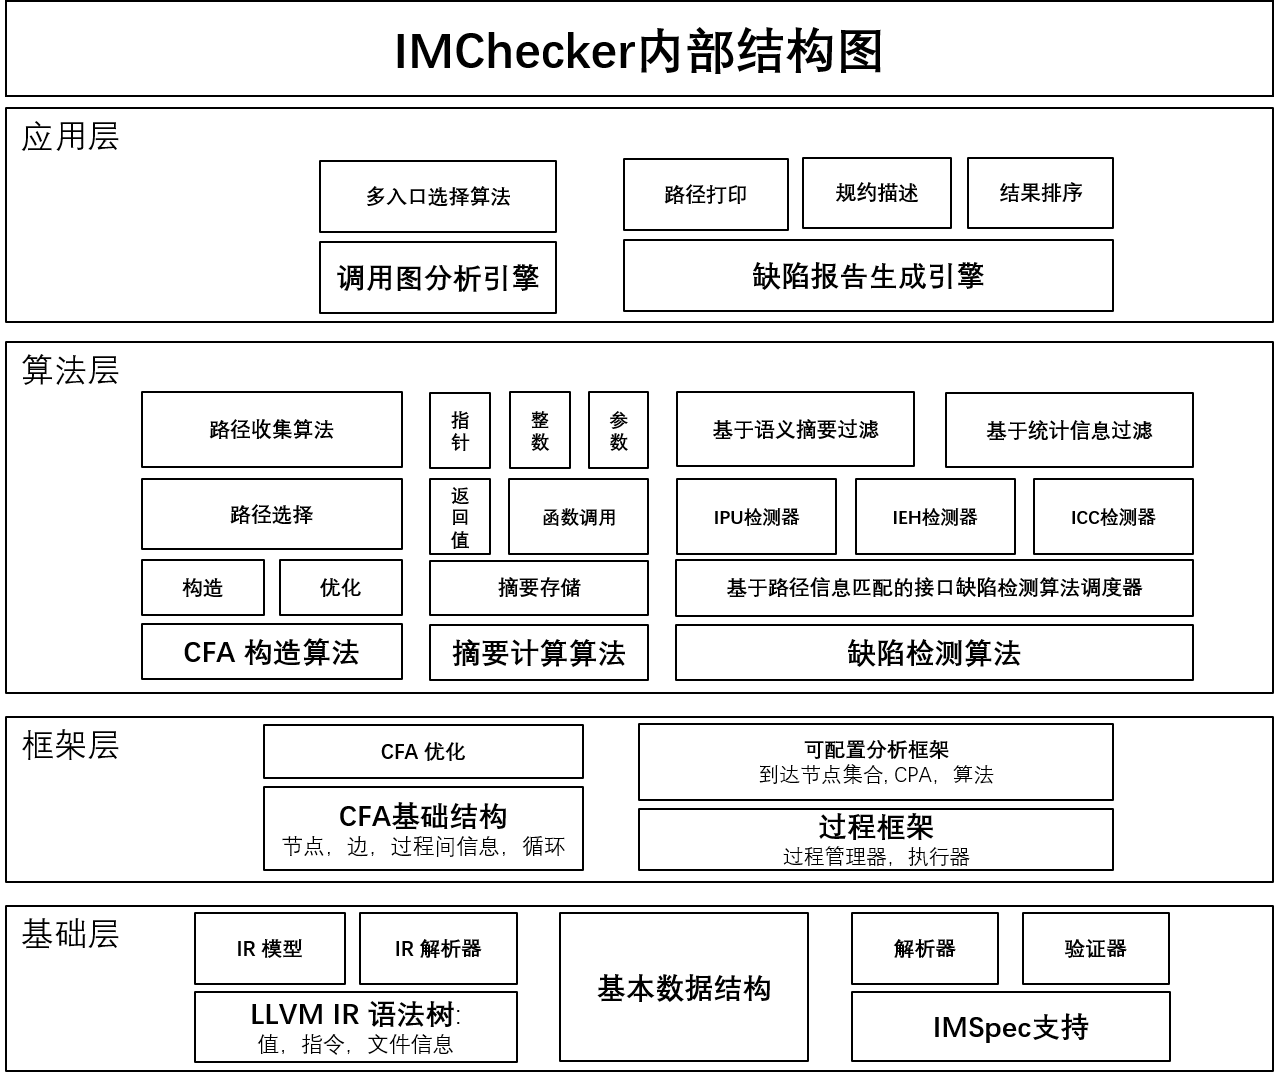
\includegraphics[width=0.9\linewidth]{figures/cp3-implementation.png}
	\caption{
		IMChecker工具内部结构图
	}
	\label{fig:3-4-implementation}
\end{figure}

\subsection{工具实现}
IMChecker基于Java语言实现,依赖于LLVM3.9的IR作为分析的中间表达,
并基于CPA~\cite{07-cav-cpachecker}算法作为整体方法的实现基础。
工具实现的内部结构如图~\ref{fig:3-4-implementation}所示。
工具共包含四个层次:基础层、架构层、算法层和应用层。
首先,基础层通过对源代码处理,生成LLVM-IR中间表达;并对IMSpec规约描述进行解析和一致性分析。
架构层构造CFA,将程序转化为图结构;
同时,提供基于CPA算法的分析流程以支持上层语义计算的算法。
算法层,则对CFA进行优化、计算语义摘要信息以及缺陷检测。
最后,应用层通过调用图具体进行分析入口的选择,执行缺陷分析;
并将缺陷检测的结果进行过滤、排序和信息打印。

\paragraph{基础层}
基础层旨在对用于输入的源代码和IMSpec规约描述进行预处理,同时提供分析中需要的基本数据机构。
首先,针对于用户输入的源代码,
如果待测程序是单个的C文件,IMChecker直接使用clang编译器
\begin{lstlisting}[language={bash},
basicstyle=\linespread{0.8}\listingsfont,
numbers=none,
xleftmargin=.25\textwidth]
(*@\textcolor{blue}{Ubuntu@~: clang}@*) path2source -S -emit-llvm -g
\end{lstlisting}
进行预处理以生成自包含的.ll文件。
该文件相比于原.c文件增加了必需的函数和数据结构声明,展开了宏定义,消去了预处理指令等。
同时生成了对应的LLVM-IR中间表达。
如果待测程序是一个Makefile工程,
那么通过解析Makefile中的编译指令并且将所有输出.o文件的指令替换为相应的预处理指令,例如clang -E。
预处理生成的.i文件,再利用上述指令生成.ll文件。
同时,根据Makefile的编译目标,项目被组织成不同的分析任务。
通过llvm的链接指令(llvm-link)将给定分析任务下所有的.ll文件进行合并,
作为输入进行缺陷检测。
在获得LLVM-IR中间表达后,利用javacpp\footnote{https://github.com/bytedeco/javacpp}工具解析文件,
并构造IR模型,包括值、指令和文件信息。
另一方面,基础层对用户提供的IMSpec语言进行解析。
IMSpec语言针对于单个目标API设计,所以如果规约中存在语法错误则将错误规约忽略并输出给使用者。
同时,解析后的IMSpec进行语义一致性验证,即是否存在冲突的约束。
例如,一个条件未接口的第一个参数大于零,另一个条件未第一个参数小于零等等。

\paragraph{框架层}
框架层旨在提供分析框架的实现以及基本土结构的创建。
在对用户提供的源代码解析过后,CFA基本结构模块对LLVM-IR进行包装,构造CFA结构。
特别地,CFA在节点上表示程序的位置,在边上封装程序的具体执行指令。
为了在CFA图上提供更多的语义信息,
本文将CFA边分为两种,即控制边和摘要边。
前者表示具体的语义操作的指令,例如存储、运算、返回等等。
后者表示函数调用和循环关系。
因此,通过摘要边,在分析中可以利用摘要信息跳过函数展开和循环遍历,
在保证大规模代码有效分析的同时增加分析精度。


\paragraph{算法层}

\paragraph{应用层}


目前,IMChecker已经集成在Tsmart工具集中~\cite{tsmart},工具使用的具体细节将在第~\ref{sec:4.3}中进行介绍。
\subsection{实验环境介绍}
测试集合

每类特点介绍
1页
比较对象
0.5
\subsection{评测结果}
imchecker imchecker--

imchecker和其他

详细分析

结果表格解释1页

自己工具每个分类的情况2页,误报、漏报原因

其他工具对比2页


\section{本章小结}
\label{sec:3.5}
本章提出了基于缺陷描述的规模化接口缺陷静态检测技术IMChecker。
IMChecker利用IMSpec语言对接口使用约束进行描述,以支持用户自己定义的接口。
同时,IMChecker基于多入口分析,将复杂的程序分析问题分而治之,高效率分析的同时,
实现局部的精确分析。
对于多入口分析策略引入的精度损失而导致的误报,
IMChecker通过基于上下文语义的摘要信息和基于使用情况的统计信息对结果进行过滤,以提交检测精度。
在Juliet Test Suite的13个接口缺陷相关的评测集上的实验结果显示,
IMCHecker方法误报率为13.21\%,漏报率为16.08\%。
检测能力领先于主流的开源软件项目。
